% ================================================================
\chapter{Listas de prioridades e heaps binários}\label{cap:heap}\label{sec:heap}
% ================================================================
\begin{objetivos}
\begin{itemize}
  \item O tipo abstrato lista de prioridades e o custo de implementá-lo com listas.
  \item O heap binário: definição, representação em vetor e as operações \emph{subir} e \emph{descer}.
  \item Inserção, remoção e alteração de prioridade em $O(\log n)$, e construção em $O(n)$.
  \item O heapsort e as técnicas para demonstrar propriedades de heaps.
\end{itemize}
\end{objetivos}

Muitas aplicações precisam, repetidamente, do elemento \emph{mais importante} de uma coleção que muda o tempo todo: o próximo processo a ser executado, o paciente mais grave de uma emergência, o próximo evento de uma simulação, o vértice mais próximo no algoritmo de Dijkstra. O tipo abstrato que atende a essas aplicações é a \textbf{lista de prioridades}, e sua implementação clássica é o \textbf{heap binário}: um vetor com uma ordem parcial que permite todas as operações em tempo logarítmico e a construção em tempo linear.

\section{Listas de prioridades}\label{sec:listaprior}
Uma lista de prioridades é uma tabela em que cada elemento tem uma \textbf{prioridade}, e que oferece as operações de
\begin{itemize}
  \item \emph{seleção} do elemento de maior prioridade;
  \item \emph{inserção} de um novo elemento;
  \item \emph{remoção} do elemento de maior prioridade;
  \item \emph{alteração} da prioridade de um elemento;
  \item \emph{construção} da tabela a partir de um conjunto inicial.
\end{itemize}
A operação de \emph{fusão} de duas listas será tratada no Capítulo~\ref{cap:heapav}.

\begin{exemplo}[A fila de um pronto-socorro]\label{ex:prontosocorro}
Num pronto-socorro, cada paciente recebe uma nota de gravidade de 0 a 100 na triagem. Uma sequência típica de eventos é:
\begin{center}\small
\begin{tabular}{@{}ll@{}}
\toprule
evento & operação\\
\midrule
chegam Ana (40), Bruno (75) e Carla (20) & construção com $\{40,75,20\}$\\
o médico fica livre & seleção e remoção: atende Bruno (75)\\
chega Davi (90) & inserção de 90\\
o estado de Carla piora para 95 & alteração: $20\to95$\\
o médico fica livre & seleção e remoção: atende Carla (95)\\
\bottomrule
\end{tabular}
\end{center}
Note que nunca precisamos da ordem completa dos pacientes, apenas de quem é o \emph{primeiro}. É essa observação que o heap explora.
\end{exemplo}

As implementações mais simples são listas. Numa lista não ordenada, inserir é imediato, mas achar o máximo exige percorrer tudo; numa lista ordenada, o máximo está no início, mas cada inserção precisa encontrar a posição certa e deslocar elementos. Por exemplo, inserir 50 na lista ordenada $[90,70,40,20]$ exige deslocar o 40 e o 20 uma posição para a direita, e no pior caso (inserir um novo máximo) todos os elementos se deslocam. A tabela compara essas opções com o heap.
\begin{center}
\small
\begin{tabular}{@{}lccc@{}}
\toprule
Operação & Lista não ordenada & Lista ordenada & Heap\\
\midrule
seleção & $\Theta(n)$ & $\Theta(1)$ & $O(1)$\\
inserção & $\Theta(1)$ & $\Theta(n)$ & $O(\log n)$\\
remoção & $\Theta(n)$ & $\Theta(1)$ & $O(\log n)$\\
alteração & $\Theta(n)$ & $\Theta(n)$ & $O(\log n)$\\
construção & $\Theta(n)$ & $\Theta(n\log n)$ & $O(n)$\\
\bottomrule
\end{tabular}
\end{center}
Cada lista tem alguma operação de atualização que custa $\Omega(n)$. O heap abre mão de manter a ordem total e mantém só o necessário para que o máximo esteja sempre num lugar conhecido; com isso, todas as operações ficam logarítmicas.

\section{Definição e representação}\label{sec:heapdef}
\begin{intuicao}
Pense num organograma em que cada chefe é mais importante que seus subordinados diretos. Quem está no topo é o mais importante de todos, mas nada se exige entre colegas do mesmo nível, nem entre pessoas de departamentos diferentes. Um heap é exatamente isso: uma hierarquia em que \emph{cada pai domina os seus filhos}, e nada mais.
\end{intuicao}

\begin{defi}[Heap]
Um \textbf{heap} (de máximo) é uma sequência $s_1,\dots,s_n$ tal que
\[
s_i\le s_{\floor{i/2}}\qquad\text{para todo }1<i\le n .
\]
Num heap \emph{de mínimo}, a desigualdade é invertida: $s_i\ge s_{\floor{i/2}}$.
\end{defi}
A definição fica clara quando se desenha a sequência como uma \textbf{árvore binária completa}, numerada por níveis e, em cada nível, da esquerda para a direita: o nó $i$ tem pai $\floor{i/2}$, filho esquerdo $2i$ e filho direito $2i+1$ (quando esses índices são $\le n$). A condição diz que \emph{cada nó tem prioridade maior ou igual à de seus filhos}. Não há ponteiros: a árvore é só uma maneira de olhar para o vetor (Figura~\ref{fig:heaprep}).

\begin{figura}[O mesmo heap visto como árvore e como vetor. Os números pequenos são os índices; os filhos do nó $i$ estão nas posições $2i$ e $2i+1$, como indicam as setas desenhadas junto ao vetor.\label{fig:heaprep}]
\begin{forest} bst
[90,label={[font=\tiny]above:1}, s sep=16mm
  [55,label={[font=\tiny]left:2} [41,label={[font=\tiny]left:4} [37,label={[font=\tiny]left:8}] [,vazio]] [30,label={[font=\tiny]right:5}]]
  [82,label={[font=\tiny]right:3} [64,label={[font=\tiny]left:6}] [75,label={[font=\tiny]right:7}]]]
\end{forest}
\qquad
\begin{tikzpicture}[baseline=-1.2cm,x=7mm]
\foreach \x [count=\i] in {90,55,82,41,30,64,75,37} {\node[cel] (c\i) at (\i,0) {\x}; \node[idx] at (\i,0.5) {\i};}
\draw[seta, MidnightBlue!70, bend right=50] (c1.south) to (c2.south);
\draw[seta, MidnightBlue!70, bend right=50] (c1.south) to (c3.south);
\draw[seta, BrickRed!70, bend right=45] (c2.south) to (c4.south);
\draw[seta, BrickRed!70, bend right=45] (c2.south) to (c5.south);
\draw[seta, ForestGreen!70, bend left=40] ($(c3.north)+(0,3.2mm)$) to ($(c6.north)+(0,3.2mm)$);
\draw[seta, ForestGreen!70, bend left=40] ($(c3.north)+(0,3.2mm)$) to ($(c7.north)+(0,3.2mm)$);
\end{tikzpicture}
\end{figura}

\begin{exemplo}[Reconhecendo um heap]\label{ex:ehheap}
Para verificar se uma sequência é um heap, basta comparar cada posição $i\ge2$ com o seu pai $\floor{i/2}$.
\begin{itemize}
  \item $[9,7,8,3,5,6]$: os pares (filho, pai) são $(7,9)$, $(8,9)$, $(3,7)$, $(5,7)$ e $(6,8)$; em todos o filho é menor. É um heap.
  \item $[9,5,8,6,4,7]$: a posição 4 guarda $6$ e o seu pai, a posição 2, guarda $5$. Como $6>5$, \textbf{não} é um heap (Figura~\ref{fig:naoheap}). Todos os outros pares estão corretos: basta uma violação.
\end{itemize}
Observe que no heap $[9,7,8,3,5,6]$ os irmãos 7 e 8 aparecem em ordem crescente, e o 6, à direita, é maior que o 3 e o 5, à esquerda: nada disso importa. Só se comparam pais e filhos.
\begin{figura}[À esquerda, um heap. À direita, uma sequência que não é heap: a aresta em vermelho liga o pai 5 a um filho maior, 6.\label{fig:naoheap}]
\begin{forest} bstp
[9 [7 [3] [5]] [8 [6] [,vazio]]]
\end{forest}
\hspace{2cm}
\begin{forest} bstp
[9 [5,desreg [6,aviol,desreg] [4]] [8 [7] [,vazio]]]
\end{forest}
\end{figura}
\end{exemplo}

Alguns fatos sobre os índices aparecem em todas as demonstrações deste capítulo:
\begin{itemize}
  \item o nó $i$ está no nível $\floor{\log_2i}+1$ (a raiz está no nível 1), e a árvore tem $\floor{\log_2n}+1$ níveis;
  \item o nó $i$ tem filho se e somente se $2i\le n$; logo as \textbf{folhas} são exatamente as posições $\floor{n/2}+1,\dots,n$, e há $\ceil{n/2}$ delas;
  \item neste capítulo, a altura de um nó é medida em níveis: \textbf{folhas têm altura 1}.
\end{itemize}

\begin{exemplo}[Fazendo contas com índices]\label{ex:indices}
Num heap com $n=10$ elementos: o pai do nó $7$ é $\floor{7/2}=3$; os filhos do nó $4$ são $8$ e $9$; o nó $5$ tem só o filho esquerdo $10$, pois $11>n$; as folhas são as posições $6,\dots,10$ (são $\ceil{10/2}=5$ folhas); o nó $9$ está no nível $\floor{\log_29}+1=4$, e a árvore tem $\floor{\log_210}+1=4$ níveis.
\end{exemplo}

\section{As operações subir e descer}\label{sec:subirdescer}
Toda operação sobre um heap altera uma posição e depois restaura a propriedade de heap, que pode ter sido violada em apenas um ponto:
\begin{itemize}
  \item se a prioridade de um nó \emph{aumentou}, ele pode ter ficado maior que o pai, e precisa \textbf{subir};
  \item se \emph{diminuiu}, pode ter ficado menor que um filho, e precisa \textbf{descer}.
\end{itemize}

\begin{pseudo}{subir$(i)$ -- após \emph{aumentar} a prioridade de $i$}
\begin{algorithmic}
\Procedure{subir}{$i$}
  \State $j := \floor{i/2}$
  \If{$j\ge1$}
    \If{$T[i].chave > T[j].chave$}
      \State $T[i]\Leftrightarrow T[j]$
      \State \Call{subir}{$j$}
    \EndIf
  \EndIf
\EndProcedure
\end{algorithmic}
\end{pseudo}
\begin{pseudo}{descer$(i,n)$ -- após \emph{diminuir} a prioridade de $i$}
\begin{algorithmic}
\Procedure{descer}{$i,n$}
  \State $j := 2i$
  \If{$j\le n$}
    \If{$j<n$ \textbf{e} $T[j+1].chave > T[j].chave$}
      \State $j := j+1$ \Comment{maior filho}
    \EndIf
    \If{$T[i].chave < T[j].chave$}
      \State $T[i]\Leftrightarrow T[j]$
      \State \Call{descer}{$j,n$}
    \EndIf
  \EndIf
\EndProcedure
\end{algorithmic}
\end{pseudo}
Ambos percorrem um único caminho da árvore, logo custam $O(\log n)$. Um detalhe essencial do \emph{descer} é que ele troca o nó com o \textbf{maior} dos filhos: se trocasse com o menor, o maior filho ficaria abaixo de um valor menor que ele, e a propriedade continuaria violada.

\begin{exemplo}[Por que trocar com o maior filho]
Suponha que a raiz de $[4,9,7]$ precise descer. Trocando com o maior filho, 9, obtemos $[9,4,7]$, um heap. Trocando com o menor, 7, obteríamos $[7,9,4]$, e agora o filho 9 é maior que o pai 7: a violação não foi corrigida, só mudou de lugar.
\end{exemplo}

\section{Inserção, remoção e alteração de prioridade}\label{sec:heapops}
Com \emph{subir} e \emph{descer}, as demais operações são imediatas:
\begin{itemize}
  \item para \textbf{inserir}, o novo elemento ocupa a primeira posição livre do vetor, a $n+1$, e sobe;
  \item para \textbf{remover o máximo}, o último elemento é copiado para a raiz e desce;
  \item para \textbf{alterar} uma prioridade, o elemento sobe ou desce conforme a prioridade tenha aumentado ou diminuído.
\end{itemize}
Em todos os casos o \emph{formato} da árvore continua o de uma árvore completa (só a última posição é criada ou apagada), e a ordem é consertada ao longo de um único caminho.
\begin{pseudo}{Inserção, remoção do máximo e alteração de prioridade}
\begin{algorithmic}
\Procedure{inserir}{$novo$} \Comment{$M$ é a capacidade do vetor}
  \If{$n<M$} \State $T[n+1]:=novo$;\ $n:=n+1$;\ \Call{subir}{$n$}
  \Else\ \textbf{overflow}
  \EndIf
\EndProcedure
\Procedure{remover}{}
  \If{$n\ne0$} \State processar$(T[1])$;\ $T[1]:=T[n]$;\ $n:=n-1$;\ \Call{descer}{$1,n$}
  \Else\ \textbf{underflow}
  \EndIf
\EndProcedure
\Procedure{alterar}{$i, p$}
  \State $antiga := T[i].chave$;\ $T[i].chave := p$
  \If{$p > antiga$} \State \Call{subir}{$i$} \Comment{aumentou: sobe}
  \Else \State \Call{descer}{$i,n$} \Comment{diminuiu: desce}
  \EndIf
\EndProcedure
\end{algorithmic}
\end{pseudo}

\begin{exemplo}[Inserção passo a passo]\label{ex:heapins}
Inserimos 68 no heap $[90,55,82,41,30,64,75,37]$ da Figura~\ref{fig:heaprep}. Ele entra na posição 9, como filho de 41. Como $68>41$, troca com o pai; na posição 4, $68>55$, e troca de novo; na posição 2, $68<90$, e para. O resultado é $[90,68,82,55,30,64,75,37,41]$. Foram duas trocas, ao longo do caminho de uma folha até a raiz.
\begin{figura}[Inserção de 68: o novo elemento (em destaque) entra na primeira posição livre e sobe enquanto for maior que o pai. A aresta azul é a comparação seguinte.\label{fig:heapins}]
\begin{tabular}{@{}c@{\hspace{6mm}}c@{\hspace{6mm}}c@{}}
\begin{forest} bstp
[90 [55 [41 [37] [68,novo,acam]] [30]] [82 [64] [75]]]
\end{forest} &
\begin{forest} bstp
[90 [55 [68,novo,acam [37] [41]] [30]] [82 [64] [75]]]
\end{forest} &
\begin{forest} bstp
[90 [68,novo,acam [55 [37] [41]] [30]] [82 [64] [75]]]
\end{forest}\\
\small (a) entra na posição 9 & \small (b) troca com 41 & \small (c) troca com 55; $68<90$: fim
\end{tabular}
\end{figura}
\end{exemplo}

\begin{exemplo}[Remoção passo a passo]\label{ex:heaprem}
Removemos o máximo de $H=[90,55,82,\allowbreak41,30,\allowbreak64,75,37]$. O último elemento, 37, vai para a raiz, formando $[37,55,82,41,30,64,75]$. Agora 37 desce: os filhos são 55 e 82, e ele troca com o maior, 82; na posição 3, os filhos são 64 e 75, e ele troca com 75; na posição 7, é folha, e para. Resultado: $[82,55,75,41,30,64,37]$.
\begin{figura}[Remoção do máximo: o último elemento ocupa a raiz e desce, sempre trocando com o maior filho.\label{fig:heaprem}]
\begin{tabular}{@{}c@{\hspace{8mm}}c@{\hspace{8mm}}c@{}}
\begin{forest} bstp
[37,novo [55 [41] [30]] [82,acam [64] [75]]]
\end{forest} &
\begin{forest} bstp
[82 [55 [41] [30]] [37,novo [64] [75,acam]]]
\end{forest} &
\begin{forest} bstp
[82 [55 [41] [30]] [75 [64] [37,novo]]]
\end{forest}\\
\small (a) 37 vai para a raiz & \small (b) troca com 82 & \small (c) troca com 75: fim
\end{tabular}
\end{figura}
\end{exemplo}

\begin{exemplo}[Alteração de prioridade]\label{ex:heapalt}
No mesmo heap $H=[90,55,82,41,30,64,75,37]$:
\begin{itemize}
  \item \textbf{aumentar} a prioridade do nó 6 de 64 para 95: ele sobe trocando com 82 (posição 3) e com 90 (posição 1), e o heap fica $[95,55,90,41,$\allowbreak$30,82,75,37]$;
  \item \textbf{diminuir} a raiz de 90 para 33: ela desce trocando com 82 e com 75: $[82,55,75,41,$\allowbreak$30,64,33,37]$.
\end{itemize}
\end{exemplo}

\begin{cuidado}[Subir ou descer?]
É comum inverter as duas operações ao alterar uma prioridade, escrevendo algo como ``\textbf{se} $H[i]>H[\floor{i/2}]$ \textbf{então} descer$(i)$ \textbf{senão} subir$(i)$''. O correto é o contrário: se o novo valor ficou maior que o pai, a violação é \emph{com o pai}, e o elemento precisa \textbf{subir}; se não ficou, a única violação possível é com os filhos, e ele precisa \textbf{descer}. Em pseudocódigo: \textbf{se} $i>1$ \textbf{e} $H[i]>H[\floor{i/2}]$ \textbf{então} subir$(i)$ \textbf{senão} descer$(i,n)$.
\end{cuidado}

\section{Construção em tempo linear}\label{sec:arranjar}
Para transformar um vetor arbitrário num heap, a primeira ideia é inseri-lo elemento a elemento: \textbf{para} $i:=2,\dots,n$ \textbf{faça} subir$(i)$. Isso custa $O(n\log n)$, e de fato $\Theta(n\log n)$ no pior caso, por exemplo quando a entrada é crescente e cada elemento sobe até a raiz.

Uma ideia melhor é trabalhar de baixo para cima. As folhas, isto é, as posições $i>\floor{n/2}$, já são heaps de um único elemento. Percorrendo os demais nós do último para o primeiro, cada um encontra as duas subárvores dos filhos já organizadas como heaps, e basta fazê-lo descer.
\begin{pseudo}{arranjar$(n)$: construção do heap}
\begin{algorithmic}
\Procedure{arranjar}{$n$}
  \For{$i := \floor{n/2}$ \textbf{decrescendo até} $1$} \State \Call{descer}{$i,n$} \EndFor
\EndProcedure
\end{algorithmic}
\end{pseudo}
A correção segue do invariante ``antes de processar $i$, as subárvores com raízes $i+1,\dots,n$ são heaps''.

\begin{exemplo}[O \emph{arranjar} passo a passo]\label{ex:arranjar}
Construímos um heap a partir de $[5,13,8,2,11,9,14]$, com $n=7$. As folhas são as posições $4,\dots,7$; processamos $i=3,2,1$ (Figura~\ref{fig:arranjar}).
\begin{itemize}
  \item $i=3$ (valor 8): os filhos são 9 e 14; troca com 14. Vetor: $[5,13,14,2,11,9,8]$.
  \item $i=2$ (valor 13): os filhos são 2 e 11, ambos menores; nada muda.
  \item $i=1$ (valor 5): os filhos são 13 e 14; troca com 14, e na posição 3 os filhos são 9 e 8; troca com 9. Vetor final: $[14,13,9,2,11,5,8]$.
\end{itemize}
\begin{figura}[O \emph{arranjar} sobre $[5,13,8,2,11,9,14]$. Em cada passo, o nó processado (em destaque) desce enquanto for menor que o maior filho; as subárvores abaixo dele já são heaps.\label{fig:arranjar}]
\begin{tabular}{@{}c@{\hspace{7mm}}c@{\hspace{7mm}}c@{\hspace{7mm}}c@{}}
\begin{forest} bstp
[5 [13 [2] [11]] [8,novo [9] [14]]]
\end{forest} &
\begin{forest} bstp
[5 [13,novo [2] [11]] [14 [9] [8]]]
\end{forest} &
\begin{forest} bstp
[5,novo [13 [2] [11]] [14 [9] [8]]]
\end{forest} &
\begin{forest} bstp
[14,feito [13,feito [2,feito] [11,feito]] [9,feito [5,feito] [8,feito]]]
\end{forest}\\
\small (a) $i=3$ & \small (b) $i=2$: nada muda & \small (c) $i=1$ & \small (d) heap pronto
\end{tabular}
\end{figura}
\end{exemplo}

O ponto surpreendente é o custo: a maioria dos nós está perto das folhas e desce pouco. A Figura~\ref{fig:alturas} mostra a conta numa árvore cheia com 15 nós.
\begin{figura}[Numa árvore completa, metade dos nós são folhas e não descem nada; um quarto desce no máximo um nível; e assim por diante. Com 15 nós, o \emph{arranjar} faz no máximo $4\cdot1+2\cdot2+1\cdot3=11$ trocas, menos que $n$.\label{fig:alturas}]
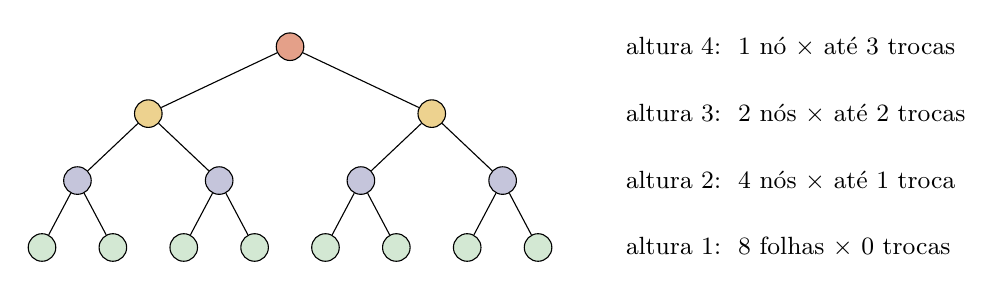
\begin{tikzpicture}[x=0.9cm,y=0.85cm]
\foreach \d/\cor in {0/BrickRed!35,1/Goldenrod!50,2/MidnightBlue!25,3/ForestGreen!20} {
  \pgfmathtruncatemacro{\m}{2^\d}
  \foreach \k in {1,...,\m} {\node[circle,draw,fill=\cor,minimum size=3.5mm,inner sep=0pt] (n\d-\k) at ({(\k-0.5)*8/\m},-\d) {};}}
\foreach \d in {1,2,3} {
  \pgfmathtruncatemacro{\p}{\d-1}\pgfmathtruncatemacro{\m}{2^\d}
  \foreach \k in {1,...,\m} {\pgfmathtruncatemacro{\q}{(\k+1)/2}\draw (n\p-\q) -- (n\d-\k);}}
\foreach \d/\txt in {0/{altura 4:\ \ 1 nó $\times$ até 3 trocas},1/{altura 3:\ \ 2 nós $\times$ até 2 trocas},2/{altura 2:\ \ 4 nós $\times$ até 1 troca},3/{altura 1:\ \ 8 folhas $\times$ 0 trocas}}
  {\node[anchor=west,font=\small] at (8.6,-\d) {\txt};}
\end{tikzpicture}
\end{figura}

\begin{lema}\label{lema:alturas}
Numa árvore binária completa com $n$ nós (folhas com altura 1), no máximo $\ceil{n/2^j}$ nós têm altura $j$.
\end{lema}
\begin{proof}
Numa árvore completa, o caminho mais longo que desce de $i$ é o da esquerda: $i\to2i\to4i\to\cdots$. Logo o nó $i$ tem altura $\ge j$ se e somente se o seu descendente $j-1$ níveis abaixo existe, isto é, $i\,2^{j-1}\le n$, ou $i\le\floor{n/2^{j-1}}$. Assim, com $x=n/2^{j-1}$ e $m=\floor{x}$,
\[
\#\{\text{altura}=j\}=\floor{x}-\floor{x/2}=m-\floor{m/2}=\ceil{m/2}\le\ceil{x/2}=\ceil{n/2^j}.\qedhere
\]
\end{proof}

\begin{teo}
O procedimento arranjar$(n)$ roda em tempo $O(n)$.
\end{teo}
\begin{proof}
Num nó de altura $j$, descer faz no máximo $j-1$ trocas. Pelo Lema~\ref{lema:alturas}, o total de trocas é
\[
\sum_{j=2}^{h}(j-1)\ceil*{\frac{n}{2^j}}\ \le\ \sum_{j\ge2}(j-1)\Bigl(\frac{n}{2^j}+1\Bigr)
\ =\ n\sum_{j\ge2}\frac{j-1}{2^j}+O(\log^2 n)\ =\ n+O(\log^2n)=O(n),
\]
pois $\sum_{j\ge1}\frac{j-1}{2^j}=\sum_{j\ge1}\frac{j}{2^j}-\sum_{j\ge1}\frac1{2^j}=2-1=1$.
\end{proof}
A intuição é a da Figura~\ref{fig:alturas}: metade dos nós (as folhas) não custa nada, um quarto custa no máximo uma troca, um oitavo no máximo duas, e assim por diante; só a raiz pode descer $\log n$ níveis. Na construção por inserções sucessivas acontece o contrário: os muitos nós de baixo são justamente os que podem subir mais.

\begin{exemplo}[Mais duas construções]\label{ex:construcoes}\leavevmode
\begin{itemize}
  \item $[12,30,21,8,$\allowbreak$27,40,16,35,19]$, com $n=9$, processa $i=4,3,2,1$. Em $i=4$, troca $8\leftrightarrow35$; em $i=3$, $21\leftrightarrow40$; em $i=2$, $30\leftrightarrow35$, e o 30 para na posição 4, pois os seus novos filhos, 8 e 19, são menores; em $i=1$, $12\leftrightarrow40$ e depois $12\leftrightarrow21$. Resultado: $[40,35,21,30,$\allowbreak$27,12,16,8,19]$.
  \item $[6,9,14,3,12,10,2]$ processa $i=3,2,1$: nada muda em $i=3$, pois 14 já é maior que 10 e 2; em $i=2$, $9\leftrightarrow12$; em $i=1$, $6\leftrightarrow14$ e depois $6\leftrightarrow10$. Resultado: $[14,12,10,3,9,6,2]$.
\end{itemize}
\end{exemplo}

\section{Heapsort}\label{sec:heapsort}
O heap leva a um algoritmo de ordenação simples: construa o heap e, repetidamente, troque a raiz (o maior elemento restante) com a última posição da parte ainda não ordenada e faça a nova raiz descer. O vetor fica dividido em duas partes: à esquerda, um heap que encolhe; à direita, a parte já ordenada, que cresce.
\begin{pseudo}{Heapsort}
\begin{algorithmic}
\Procedure{heapsort}{$T,n$}
  \State \Call{arranjar}{$n$} \Comment{$O(n)$}
  \For{$m := n$ \textbf{decrescendo até} $2$}
    \State $T[1]\Leftrightarrow T[m]$ \Comment{o máximo vai para o fim}
    \State \Call{descer}{$1, m-1$} \Comment{$O(\log m)$}
  \EndFor
\EndProcedure
\end{algorithmic}
\end{pseudo}

\begin{exemplo}[{Heapsort de $[5,2,9,4,7]$}]\label{ex:heapsort}
O \emph{arranjar} processa $i=2$ (troca $2\leftrightarrow7$) e $i=1$ (troca $5\leftrightarrow9$), e o heap é $[9,7,5,4,2]$. Em seguida, a cada passo o máximo vai para o fim e a nova raiz desce (Figura~\ref{fig:heapsort}).
\begin{figura}[Heapsort de $[5,2,9,4,7]$. A parte verde já está na posição final; a parte branca é um heap. Em cada linha, a raiz trocou de lugar com a última posição do heap e depois desceu.\label{fig:heapsort}]
\begin{tikzpicture}[x=7mm,y=7.5mm]
\foreach \lin/\vals/\k/\txt in {0/{9,7,5,4,2}/5/{heap inicial},1/{7,4,5,2,9}/4/{$9\leftrightarrow2$; o 2 desce: troca com 7 e com 4},2/{5,4,2,7,9}/3/{$7\leftrightarrow2$; o 2 desce: troca com 5},3/{4,2,5,7,9}/2/{$5\leftrightarrow2$; o 2 desce: troca com 4},4/{2,4,5,7,9}/0/{$4\leftrightarrow2$: ordenado}}{
  \foreach \x [count=\i] in \vals {
    \ifnum\i>\k \fill[feito] (\i-0.5,-\lin-0.3) rectangle (\i+0.5,-\lin+0.3); \fi
    \node[cel] at (\i,-\lin) {\x};}
  \node[rot,anchor=west] at (5.8,-\lin) {\txt};}
\end{tikzpicture}
\end{figura}
\end{exemplo}

O custo é $O(n)+\sum_mO(\log m)=\Theta(n\log n)$ em \emph{todos} os casos, mesmo com a entrada já ordenada. O heapsort é \textbf{in-place} (só faz trocas dentro do vetor) e \textbf{não é estável}, pois a troca da raiz com o último elemento pode inverter a ordem relativa de elementos iguais. Como faz $O(n\log n)$ comparações, é ótimo entre os algoritmos baseados em comparações (Capítulo~\ref{cap:sortcomp}). Por exemplo, ele transforma $[12,30,21,8,27,40,16,35,19]$ em $[8,12,16,19,21,27,30,35,40]$.

% ------------------------------------------------------------------
\section{Propriedades de heaps e suas demonstrações}\label{sec:heapprops}
\begin{roteiro}[Como demonstrar propriedades de heaps]
Quase toda demonstração sobre heaps usa só três ferramentas: (i) a definição $s_i\le s_{\floor{i/2}}$ combinada com a \textbf{transitividade ao longo de um caminho}; (ii) os \textbf{fatos sobre índices} (pai, filhos, folhas, níveis); (iii) \textbf{indução} na altura, no nível ou no número de nós. Para ``provar ou dar contraexemplo'', teste primeiro exemplos pequenos, com $n\le8$.
\end{roteiro}

\begin{prop}[O ancestral domina]\label{prop:ancestral}
Se $j$ é ancestral de $i$ num heap, então $s_i\le s_j$. Em particular, todo caminho da raiz até uma folha é não crescente, a \textbf{raiz é o máximo} e \textbf{toda subárvore é um heap}.
\end{prop}
\begin{proof}
O caminho de $i$ até $j$ é $i,\floor{i/2},\floor{i/4},\dots,j$. Aplicando a definição em cada aresta e a transitividade de $\le$, obtemos $s_i\le s_{\floor{i/2}}\le\cdots\le s_j$. A raiz é ancestral de todos os nós. A condição de heap numa subárvore é a mesma condição, restrita a ela.
\end{proof}
Por exemplo, no heap da Figura~\ref{fig:heaprep}, o caminho da raiz até a posição 8 é $90\ge55\ge41\ge37$.

\begin{prop}[O mínimo está numa folha]
Num heap de máximo com chaves distintas, o menor elemento está numa folha, isto é, numa posição maior que $\floor{n/2}$.
\end{prop}
\begin{proof}
Se $i$ não é folha, tem o filho $2i$ e $s_{2i}<s_i$, pois as chaves são distintas; logo $s_i$ não é o mínimo. Com repetições, \emph{algum} mínimo está numa folha.
\end{proof}
No heap da Figura~\ref{fig:heaprep}, as folhas são as posições $5,\dots,8$, com valores $30,64,75,37$, e o mínimo, $30$, está entre elas. Note que o mínimo pode estar em \emph{qualquer} folha, não necessariamente na última posição.

\begin{prop}[Onde está o $k$-ésimo maior]
Com chaves distintas, o $k$-ésimo maior elemento está num nível $\le k$, isto é, numa posição $\le 2^k-1$. Em particular, o segundo maior é filho da raiz (posição 2 ou 3), e o terceiro maior está entre as posições 2 e 7.
\end{prop}
\begin{proof}
Pela Proposição~\ref{prop:ancestral}, todos os ancestrais de $x$ são maiores que $x$. Se $x$ é o $k$-ésimo maior, existem só $k-1$ elementos maiores que ele, e portanto $x$ tem no máximo $k-1$ ancestrais: está no nível $\le k$. As posições dos níveis $1,\dots,k$ são $1,\dots,2^k-1$.
\end{proof}
No heap da Figura~\ref{fig:heaprep}, o segundo maior, 82, está na posição 3, e o terceiro maior, 75, na posição 7, no limite permitido.

\begin{prop}[Altura]
Um heap com $n$ elementos tem altura $\floor{\log_2 n}+1$ (em níveis), que é $\Theta(\log n)$. Por isso subir, descer, inserir e remover custam $O(\log n)$.
\end{prop}
\begin{proof}
O último nó, $n$, está no nível $\floor{\log_2n}+1$, e numa árvore completa todos os níveis anteriores estão cheios: $2^{h-1}\le n\le 2^h-1$, logo $h=\floor{\log_2n}+1$.
\end{proof}
Um heap com um milhão de elementos tem apenas $\floor{\log_2 10^6}+1=20$ níveis: nenhuma operação faz mais que 19 trocas.

\begin{prop}[Heaps e ordenação]
Toda sequência em ordem não crescente é um heap; a recíproca é falsa, como mostra $[3,1,2]$. Construir um heap é, portanto, mais fácil que ordenar: $O(n)$ contra $\Omega(n\log n)$. E, como o heapsort ordena com uma construção e $n$ remoções, nenhuma implementação de heap baseada em comparações pode ter construção \emph{e} remoção com custo amortizado $o(\log n)$; caso contrário, ordenaríamos em $o(n\log n)$.
\end{prop}

\begin{prop}[Troca de dois elementos]
Sejam $S$ um heap e $i<j$. Trocar $s_i$ com $s_j$ não produz necessariamente um heap, nem quando $s_i<s_j$ nem quando $s_i>s_j$.
\end{prop}
\begin{proof}[Contraexemplos]
Para $s_i<s_j$: $S=[10,9,1,8,7,0,0,6]$ é um heap; trocando $s_3=1$ com $s_4=8$, obtemos $[10,9,8,1,$\allowbreak$7,0,0,6]$, em que a posição 8 ($6$) tem pai na posição 4 ($1$). O valor pequeno foi para uma posição cujos filhos podem ser maiores que ele. Para $s_i>s_j$: em $S=[10,9]$, trocar as duas posições dá $[9,10]$, com o filho maior que o pai.
\end{proof}

\begin{prop}[Número de heaps]
Seja $H(n)$ o número de permutações de $1,\dots,n$ que são heaps (o mesmo vale para heaps de mínimo). Então $H(0)=H(1)=1$ e
\[
H(n)=\binom{n-1}{L}\,H(L)\,H(n-1-L),
\]
onde $L$ é o número de nós da subárvore esquerda da raiz: com $h=\floor{\log_2 n}$ e $u=n-(2^h-1)$ nós no último nível, $L=(2^{h-1}-1)+\min\{u,2^{h-1}\}$. Os valores para $n=1,\dots,10$ são $1,1,2,3,8,20,80,210,896,3360$.
\end{prop}
\begin{proof}
A raiz é necessariamente $n$. O formato da árvore é fixo, então $L$ é determinado por $n$. Escolhem-se quais $L$ dos $n-1$ valores restantes vão para a esquerda, de $\binom{n-1}{L}$ modos; cada lado precisa ser um heap sobre os seus valores, e o número de heaps depende só da quantidade de valores.
\end{proof}

\begin{exemplo}[Os três heaps de $\{1,2,3,4\}$]\label{ex:tresheaps}
Com $n=4$, a raiz é 4, a subárvore esquerda tem as posições 2 e 4 ($L=2$) e a direita, só a posição 3. Escolhemos quais 2 dos valores $\{1,2,3\}$ vão para a esquerda, de $\binom32=3$ modos, e cada escolha dá um único heap: $\{1,2\}$ dá $[4,2,3,1]$; $\{1,3\}$ dá $[4,3,2,1]$; $\{2,3\}$ dá $[4,3,1,2]$.
\end{exemplo}

\begin{prop}[Correção de subir e descer]
(a) Se $T$ era um heap e a chave de $i$ aumentou, após subir$(i)$ $T$ volta a ser um heap. (b) Se as subárvores dos filhos de $i$ são heaps, após descer$(i,n)$ a subárvore de $i$ é um heap.
\end{prop}
\begin{proof}[Esboço]
(a) Invariante: a única violação possível é entre o nó corrente e o seu pai. Ao trocar com o pai $j$, o antigo valor de $j$ desce para a posição corrente e é maior ou igual aos filhos dela, que já eram seus descendentes; o novo valor em $j$ é maior que o antigo, e não viola nada com os filhos de $j$. Repete-se para cima. (b) Invariante: a única violação é entre o nó corrente e os seus filhos. Trocando com o \emph{maior} filho, este passa a dominar o outro filho e o valor que desceu. A violação desce um nível e termina numa folha ou quando deixa de existir.
\end{proof}

\begin{chave}
Heap $=$ vetor com ``pai $\ge$ filho''. Sobe-se após um aumento e desce-se após uma diminuição, sempre trocando com o maior filho. Inserir $=$ colocar no fim e subir; remover $=$ levar o último à raiz e descer. A construção é linear porque há no máximo $\ceil{n/2^j}$ nós de altura $j$. O heapsort é $\Theta(n\log n)$, in-place e não estável.
\end{chave}

% ----------------------------------------------------------------
\section{Exercícios}
\excurso
\begin{exercicio}{hp-l1}[Lista]<ex:ehheap>
Verifique se as sequências correspondem a um heap binário (de máximo):\\
(a)~$33\ 32\ 28\ 31\ 26\ 29\ 25\ 30\ 27$;\qquad (b)~$33\ 32\ 28\ 31\ 29\ 26\ 25\ 30\ 27$.
\end{exercicio}
\begin{exercicio}{hp-l2}[Lista]<sec:heapprops>
Prove ou dê contraexemplo: se $S$ é um heap e $s_i,s_j$ são chaves com $i<j$ e $s_i<s_j$, então trocar $s_i$ com $s_j$ produz um heap.
\end{exercicio}
\begin{exercicio}{hp-l3}[Lista]<sec:heapprops>
Repita o exercício anterior com $i<j$ e $s_i>s_j$.
\end{exercicio}
\begin{exercicio}{hp-l4}[Lista]<sec:heapprops>
Determine o número de permutações de $1,\dots,n$ que são heaps de mínimo.
\end{exercicio}
\begin{exercicio}{hp-l5}[Lista]<ex:arranjar>
Aplique o algoritmo linear de construção à lista $18\ 25\ 41\ 34\ 14\ 10\ 52\ 50\ 48$.
\end{exercicio}
\begin{exercicio}{hp-l6}[Lista]<lema:alturas>
Prove que no máximo $\ceil{n/2^j}$ nós têm altura $j$ numa árvore binária completa com $n$ nós.
\end{exercicio}
\begin{exercicio}{hp-l16}[Lista]<sec:subirdescer>
Escreva os algoritmos de inserção, remoção, aumento e diminuição de prioridade e construção de heaps binários \textbf{sem recursão}.
\end{exercicio}
\begin{exercicio}{hp-r1}[Monitoria]<sec:heapdef>
(a) Defina heap e a propriedade que $s_1,\dots,s_n$ satisfazem. (b) Por que o elemento de maior prioridade é selecionado em $O(1)$? (c) Dê a complexidade de pior caso de seleção, inserção, remoção do máximo, alteração de prioridade e construção.
\end{exercicio}
\begin{exercicio}{hp-r2}[Monitoria]<sec:heapops,sec:arranjar>
No heap $H=[95,60,78,39,28,66,70,33]$: (a) a prioridade 66 passa a 98; (b) remove-se a raiz. Construa, pelo procedimento baseado em \emph{descer}, heaps a partir de (c) $[20,15,30,40,10,25,5]$ e (d) $[7,2,15,9,1,20,13]$. Mostre as trocas em cada caso.
\end{exercicio}
\begin{exercicio}{hp-r5}[Monitoria]<sec:heapops>
Um aluno escreveu: ``$H[i]:=nova$; \textbf{se} $H[i]>H[\floor{i/2}]$ \textbf{então} Descer$(i)$ \textbf{senão} Subir$(i)$''. Qual é o erro? Corrija e explique.
\end{exercicio}
\begin{exercicio}{hp-tele}[Slides]<sec:listaprior>
Problema \emph{Telemarketing} (Beecrowd 2330): $n$ vendedores, numerados de 1 a $n$, atendem $L$ ligações em ordem; cada ligação vai para o vendedor livre de menor número, que fica ocupado pela duração da ligação. Quantas ligações cada vendedor atende? Projete a solução com heap e dê a complexidade.
\end{exercicio}

\excompl
\begin{exercicio}{hp-dario}[Complementar]<sec:heapdef>
Num heap $d$-ário (cada nó tem até $d$ filhos), em vetor indexado a partir de 1: (a) quais são os índices do pai e dos filhos do nó $i$? (b) Qual a altura? (c) Quanto custam \emph{subir} e \emph{descer}? (d) Por que um $d$ maior pode ser bom quando há muito mais aumentos de prioridade do que remoções?
\end{exercicio}
\begin{exercicio}{hp-kmerge}[Complementar]<sec:heapops>
Dadas $k$ listas ordenadas com $n$ elementos no total, intercale-as numa única lista ordenada em $O(n\log k)$.
\end{exercicio}
\begin{exercicio}{hp-kmaiores}[Complementar]<sec:heapops>
Um fluxo de $n$ números chega um a um, e você tem memória $O(k)$. Como obter os $k$ maiores ao final? Qual o tempo?
\end{exercicio}
\begin{exercicio}{hp-verif}[Complementar]<ex:ehheap>
Escreva um algoritmo $O(n)$ que decide se um vetor é um heap.
\end{exercicio}
\begin{exercicio}{hp-estavel}[Complementar]<ex:heapsort>
Mostre, com um exemplo de 3 elementos, que o heapsort não é estável.
\end{exercicio}
\begin{exercicio}{hp-crescente}[Complementar]<sec:arranjar>
Mostre que construir um heap de máximo inserindo $1,2,\dots,n$, nessa ordem, por inserções sucessivas custa $\Theta(n\log n)$, enquanto o \emph{arranjar} sobre o mesmo vetor custa $O(n)$.
\end{exercicio}
\begin{exercicio}{hp-ins}[Complementar]<ex:heapins>
Insira $15,40,25,50,10,45$, nessa ordem, num heap de máximo inicialmente vazio. Mostre o vetor após cada inserção.
\end{exercicio}
\begin{exercicio}{hp-rem2}[Complementar]<ex:heaprem>
Remova o máximo duas vezes do heap $[90,70,80,30,60,50,40,10,20]$, mostrando o vetor após cada remoção.
\end{exercicio}
\begin{exercicio}{hp-sort5}[Complementar]<ex:heapsort>
Execute o heapsort sobre $[4,10,3,5,1]$, mostrando o vetor após o \emph{arranjar} e após cada passo do laço principal.
\end{exercicio}
\begin{exercicio}{hp-remi}[Complementar]<sec:heapops>
Escreva uma operação que remove o elemento da posição $i$ (não necessariamente a raiz) de um heap em $O(\log n)$. Por que, depois de pôr o último elemento na posição $i$, às vezes é preciso subir e às vezes descer?
\end{exercicio}
\begin{exercicio}{hp-mediana}[Complementar]<sec:listaprior>
Mostre como manter a mediana de um conjunto que recebe inserções, com inserção em $O(\log n)$ e consulta à mediana em $O(1)$, usando um heap de máximo e um heap de mínimo.
\end{exercicio}
\begin{exercicio}{hp-comp}[Complementar \estrela]<sec:arranjar>
Mostre que o \emph{arranjar} faz no máximo $2n$ comparações entre chaves (para $n$ grande), contando as comparações feitas em cada passo do \emph{descer}.
\end{exercicio}
